% INCLUDES PACKAGES:
% array, nomencl, etoolbox, lipsum, xmpincl, xcolor, graphicx, tabularx, 
%  makecell, subcaption, rotating, booktabs, multicol, multirow, amsmath, 
%   amsfonts, amssymb, pdflscape, textcomp, longtable, listings, pdfpages
%    xparse, ifthen, hyphenat, hyperref, cleveref, inputenc
% 
% For a full description of each of the included packages please read the 
%  packages file.

%LIST OF DEFINED SYMBOLS
        %\regTM                %Registered Trademark\regTM
        %\nonTM                %Unregistered Trademark
        %\cRight{}             %Copyright
        %\cLeft{}              %Copyleft
        %\degrees{}            %Degrees
        %\hyph{}               %Hyphen
        %\latin{<text here>}   %Latin
        %\etal{}               %et al.
        %\etc{}                %etc
        %\eg{}                 %e.g.
        %\ie{}                 %i.e.
        %\Kevlar{}             %Kevlar
        %\Matlab{}             %Matlab

%LIST OF AVAILABLE THEOREM ENVIRONMENTS
        % theorem, algorithm, axium, case, claim, conclusion, condition, 
        % conjecture, corollary, criterion, definition, example, exercise, 
        % lemma, notation, problem, proposition, remark, solution, summary
        %
        % To use:
        % \begin{<theorem name>}
        %   <YOUR TEXT HERE>
        % \end{<theorem name>}
        
%LIST OF USEFUL COMMANDS:
        %\comment{}            %Nothing inside the braces will be printed
        %\nonumeq{}            %Un-numbered, centered equation.
        %\numeq{}{label}       %Numbered, centered equation.
        %\brackS{}             %Surrounds the input with []
        %\brackR{}             %Surrounds the input with ()
        %\brackC{}             %Surrounds the input with {}

% INCLUDING CODE
	   % To include code or code snippets in your thesis, the package listings is used.
	   % A number of predefined code highlighting schemes are included in the file
	   %   listingCodeFormatting.tex including:
	   %   Matlab, C/C++, VB/VBA, and XML 
	   %
	   % Examples of how to include code are shown in Appendix C

\immediate\write18{makeindex \jobname.nlo -s nomencl.ist -o \jobname.nls}
% Write command to allow the nomenclature to be generated properly.


\documentclass[pdfa]{ualberta}
% OPTIONS FOR ualberta.cls:
% chapterbib - \printreferences now prints references at the end of a chapter
% 
% pdfa - to convert the pdfa to PDF/A format
% 
% oneside - Standard for submitting to FGSR.
% 
% twoside - If you want to print your thesis double sided.

%%%%%%%%%%%%%%%%%%%%%%%%%%%%%%%%%%%%%%%%%%%%%%%%%%%%%%%%%%%%%%%%%%%%%%%%%%%%%%%%
%                  TITLE PAGE AND FRONTMATTER INFORMATION                      %
%%%%%%%%%%%%%%%%%%%%%%%%%%%%%%%%%%%%%%%%%%%%%%%%%%%%%%%%%%%%%%%%%%%%%%%%%%%%%%%%
% TITLE PAGE INFO
 \title{This is the thesis title this is the thesis title this is the theis title this is the theis title.}              % Title of your Thesis
 \author{John Smith}        % Your Full Name
 \degree{\PhD}                     % \MSc or \PhD
 \specialization{CONTROL SYSTEMS AND ROBOTICS}                 % Leave blank if none
 \department{Electrical and Computer Engineering}   % Department you are completing your degree
 \convocationdate{Spring 2020}       % Term (Fall, Winter, Spring)

% Don't forget to edit ualberta.xmpdata with the same metadata for the PDF/A


 \abstracttext{
    Your abstract goes here ...
    
    \lipsum
 }

\preface{
This thesis is an original work by M. Ali.
    The rest of the preface goes here ...
    \lipsum
 }
\thesisquote{"Life is like riding a bicycle. To keep your balance, you must keep moving."\\- Albert Einestein}
 \dedication{
 To my mother.
 }

 \acknowledgementtext{
 Acknowledgments goes here ...
 
 \lipsum
 }

% NOMENCLATURE
% New Commands:
\newcommand\isize{0.85}
\newcommand\isizesingle{0.65}

% NOMENCLATURE
 % [A] : Constants
  % Use \nomunit{Value, Units} to add the value and units for a defined constant
 \nomenclature[A]{$c$}{Speed of light in a vacuum inertial system.\nomunit{$299,792,458\, m/s$}}
 
  % [B] : Latin
 \nomenclature[B]{$E$}{Elastic Constant (Young's Modulus)}
 
  % [C] : Greek
 \nomenclature[C]{$\alpha$}{Strain}

% ACRONYMS
    \addacronym{IoT}{Internet of Things}
    \addacronym{IIoT}{Industrial Internet of Things}
    % \addacronym{}{}
    % \addacronym{}{}
    % \addacronym{}{}
    % \addacronym{}{}
    % \addacronym{}{}
    % \addacronym{}{}
    % \addacronym{}{}
    % \addacronym{}{}
    



% BIBLIOGRAPHY LOCATION
 % .  - This folder
 % .. - Up one Folder
 \addbibresource{./References/references.bib}

%Image paths
 \graphicspath{ {./Chapters/Ch_1_Intro/images/}{./Chapters/Ch_2_Background/images/}{./Chapters/Ch_3/images/}{./Chapters/Ch_4/images/}{./Chapters/Ch_4/tempimages/}{./Chapters/Ch_x_Conlusion_FutureWork/images/}}
%%%%%%%%%%%%%%%%%%%%%%%%%%%%%%%%%%%%%%%%%%%%%%%%%%%%%%%%%%%%%%%%%%%%%%%%%%%%%%%%
%                              BEGIN DOCUMENT                                  %
%%%%%%%%%%%%%%%%%%%%%%%%%%%%%%%%%%%%%%%%%%%%%%%%%%%%%%%%%%%%%%%%%%%%%%%%%%%%%%%%
\begin{document}

 \maketitle                    % Creates the title page
 \makeabstract                 % Creates the abstract
\makepreface                  % Uncomment line to add Preface Page
 \makequote                   % Uncomment line to add Quote Page
 \makededication              % Uncomment line to add Dedication Page
 \acknowledgements             % Uncomment line to add Acknowledgements
 \tableofcontents              % Create the Table of Contents
 \listoftables                 % Uncomment line if you have tables
 \listoffigures                % Uncomment line if you have figures
%  \listofplates                 % Uncomment line if you have plates (photographs)
%  \listofsymbols               % Uncomment if you have a List of Symbols (Nomenclature)
 \abbreviations               % Uncomment if you have a List of Acronyms
 \glsaddall                    % Required for List of Acronyms and Glossary (DO NOT COMMENT)
 %\generateglossary            % Uncomment if you have Glossary
 \bodyoftext                   % Switches the style of the document to that required for the body

% SET DOCUMENT SPACING
 %\onehalfspacing        
%  \truedoublespacing
 %\triplespacing

%%%%%%%%%%%%%%%%%%%%%%%%%%%%%%%%%%%%%%%%%%%%%%%%%%%%%%%%%%%%%%%%%%%%%%%%%%%%%%%%
%                           CHAPTERS                              %
%%%%%%%%%%%%%%%%%%%%%%%%%%%%%%%%%%%%%%%%%%%%%%%%%%%%%%%%%%%%%%%%%%%%%%%%%%%%%%%%
\chapter{Introduction}\label{ch:Intro}
  \section{Motivation}\label{sec:Motivation}
    Your motivation goes here

  \section{Objectives}\label{sec:thesisObjective}
    Your objective goes here ...  
    
  \section{Outline}\label{sec:thesisOutline}
    The thesis is structured into xx main chapters as follows:
    
    In Chapter \ref{ch:background}, 
    
    Chapter \ref{ch:ch3} discusses 
    
    In Chapter \ref{ch:ch4}, 
    
    
    Finally, in Chapter \ref{ch:Conclusions}, a summary of the significant results 
\chapter{Background}\label{ch:background}
  This chapter aims to provide examples how how to structure and create specific components in your thesis document. The very first one is showing a citation, like the one at the end of this sentence \cite{patron_use_2016}. The second shows how to create more than one citation and how they are grouped \cite{zarifi_microwave_2016}.
This sentence shows how a gap in the citations is handled \cite{zarifi_time-resolved_2015}. And this book is \cite{stutzman2012antenna}. 
  \section{Tables}
  
  % L - Left Aligned (Equal Spacing)
  % C - Center Aligned (Equal Spacing)
  % R - Right Aligned (Equal Spacing)
  % l - Left Aligned (Fit to Contents)
  % c - Center Aligned (Fit to Contents)
  % r - Right Aligned (Fit to Contents)
  
  \begin{table}[!htb]
    \caption{This is a basic table}
    \centering
    \begin{tabularx}{0.75\textwidth}{LCR} 
      % Equally spaced cells that are left, center, and reight aligned. 
      % The entire table will be 75% the width of the text.
      \hline
      \textbf{Left Aligned Title} & \textbf{Centered Title} & \textbf{Right Aligned Title} \\\hline
      This is left aligned & This is centered & This is right aligned \\
      This is left aligned & This is centered & This is right aligned \\
      This is left aligned & This is centered & This is right aligned \\
      This is left aligned & This is centered & This is right aligned \\\hline
    \end{tabularx}
    \label{tab:basicTable}
  \end{table}
  
  \begin{table}[!htb]
    \caption{This is a complex table.}
    \centering
    \begin{tabularx}{\textwidth}{lCR}
      % Left most cell is fitted to the content.
      % The center and right columns are equally spaced cells that are center, and reight aligned. 
      % The entire table will be 75% the width of the text.
      \hline
      \multirow{2}{*}{\textbf{This is two row\quad}} & \multicolumn{2}{c}{\textbf{This is two columns}}\\\cline{2-3} % \cline draws a partial line across cells #-#
       & \textbf{Centered Title} & \textbf{Right Aligned Title} \\\hline
      \multirow{2}{*}{This is two row} & This is centered & This is right aligned \\
       & This is centered & This is right aligned \\\cline{1-1}
      \multirow{2}{*}{This is two row} & This is centered & This is right aligned \\
       & This is centered & This is right aligned \\\hline
    \end{tabularx}
    \label{tab:complexTable}
  \end{table}
  
  
  \section{Figures}
  This section will provide examples of how to create figures, and different types of multi/sub-figures. Additionally, if you have many figures in a section and they are bleeding too much into the following sections a \textbackslash{}clearpage command can be issued before the next section. However, note that this will force the next section to begin on a new page. Note that the first ``figure'' is actually a plate; a plate is the proper title associated with a photograph, using the environment `plate' instead of figure and command listofplates will generate everything for you.
  \begin{plate}[!htb]
    \centering
    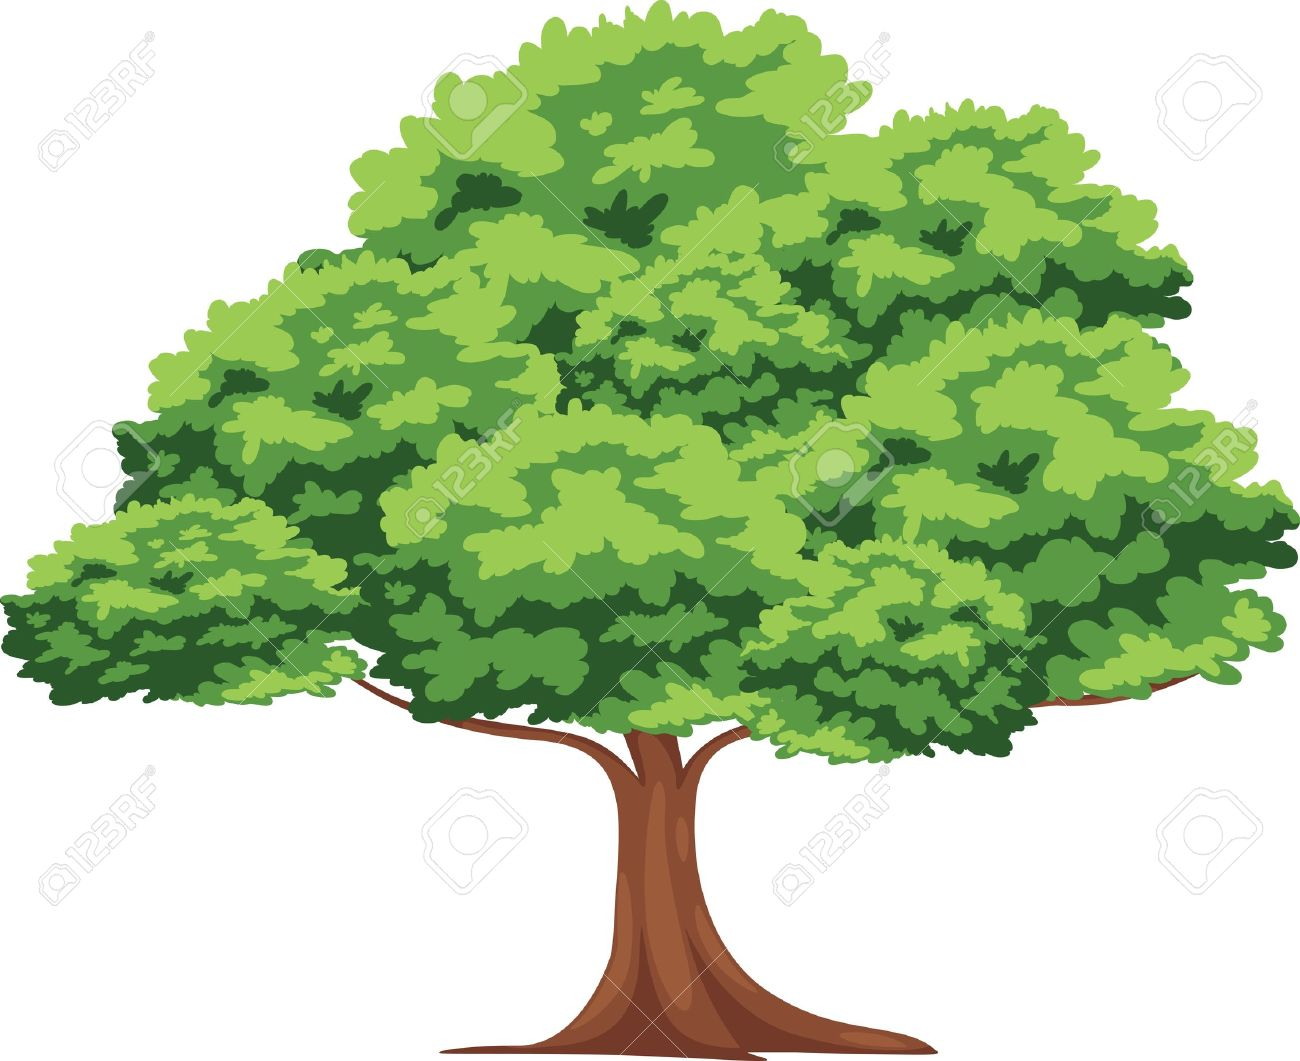
\includegraphics[width=0.7\textwidth]{sample.jpg}
    \caption{This is an example of a single image plate.}
    \label{fig1:singleImage}
  \end{plate}
  
  \begin{figure}[!htb]
    \centering
    \begin{subfigure}{0.45\textwidth}
      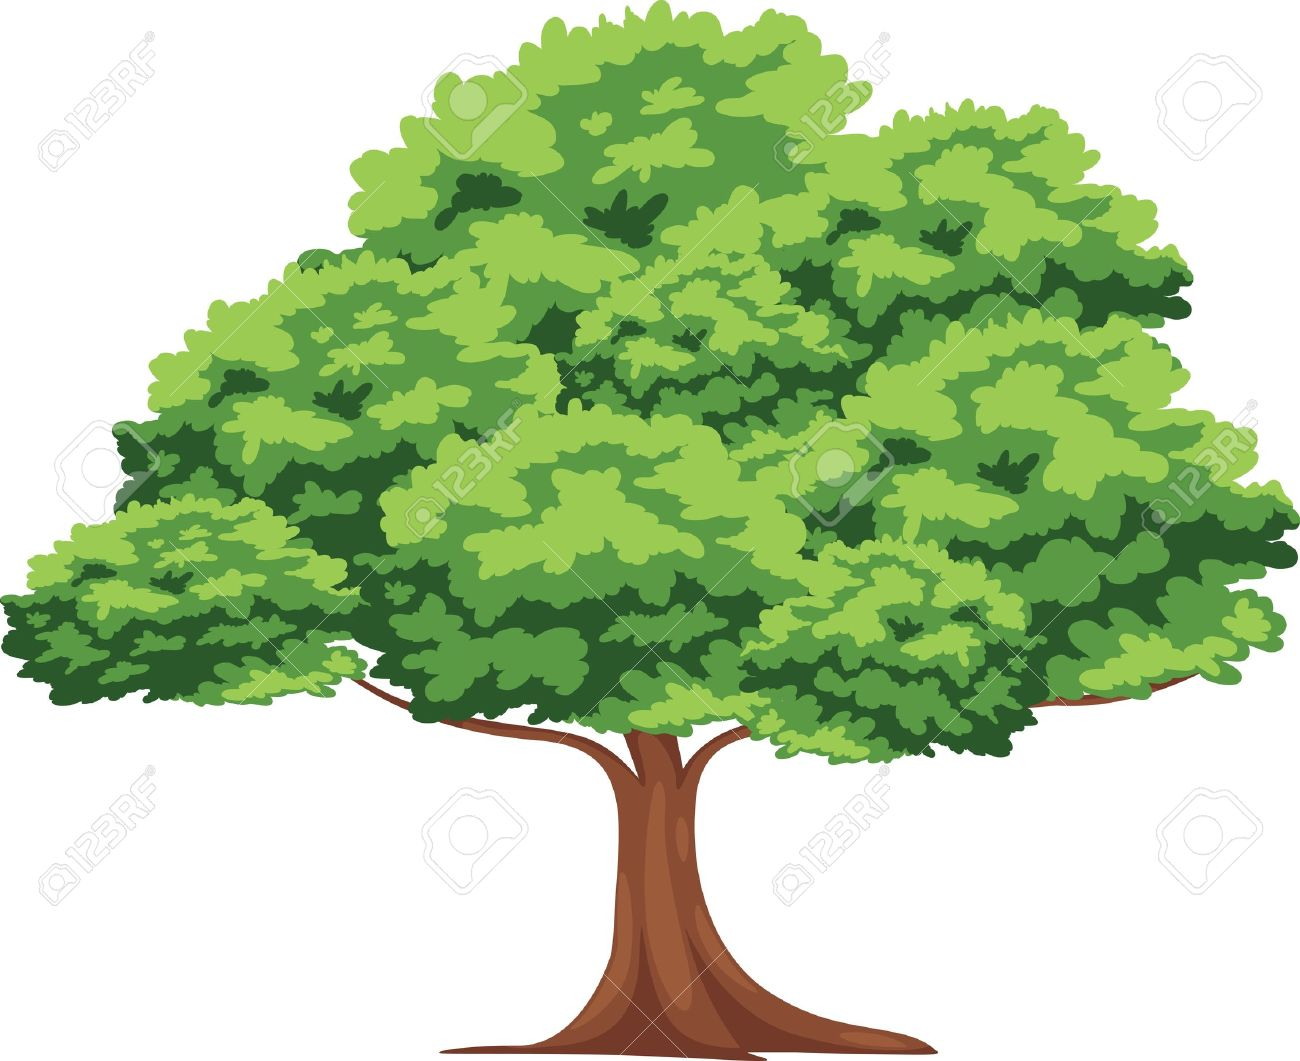
\includegraphics[width=\textwidth]{sample.jpg}
      \caption{} % Leave blank for just letter
      \label{fig2:doubleImage:a}
    \end{subfigure}
    ~
    \begin{subfigure}{0.45\textwidth}
      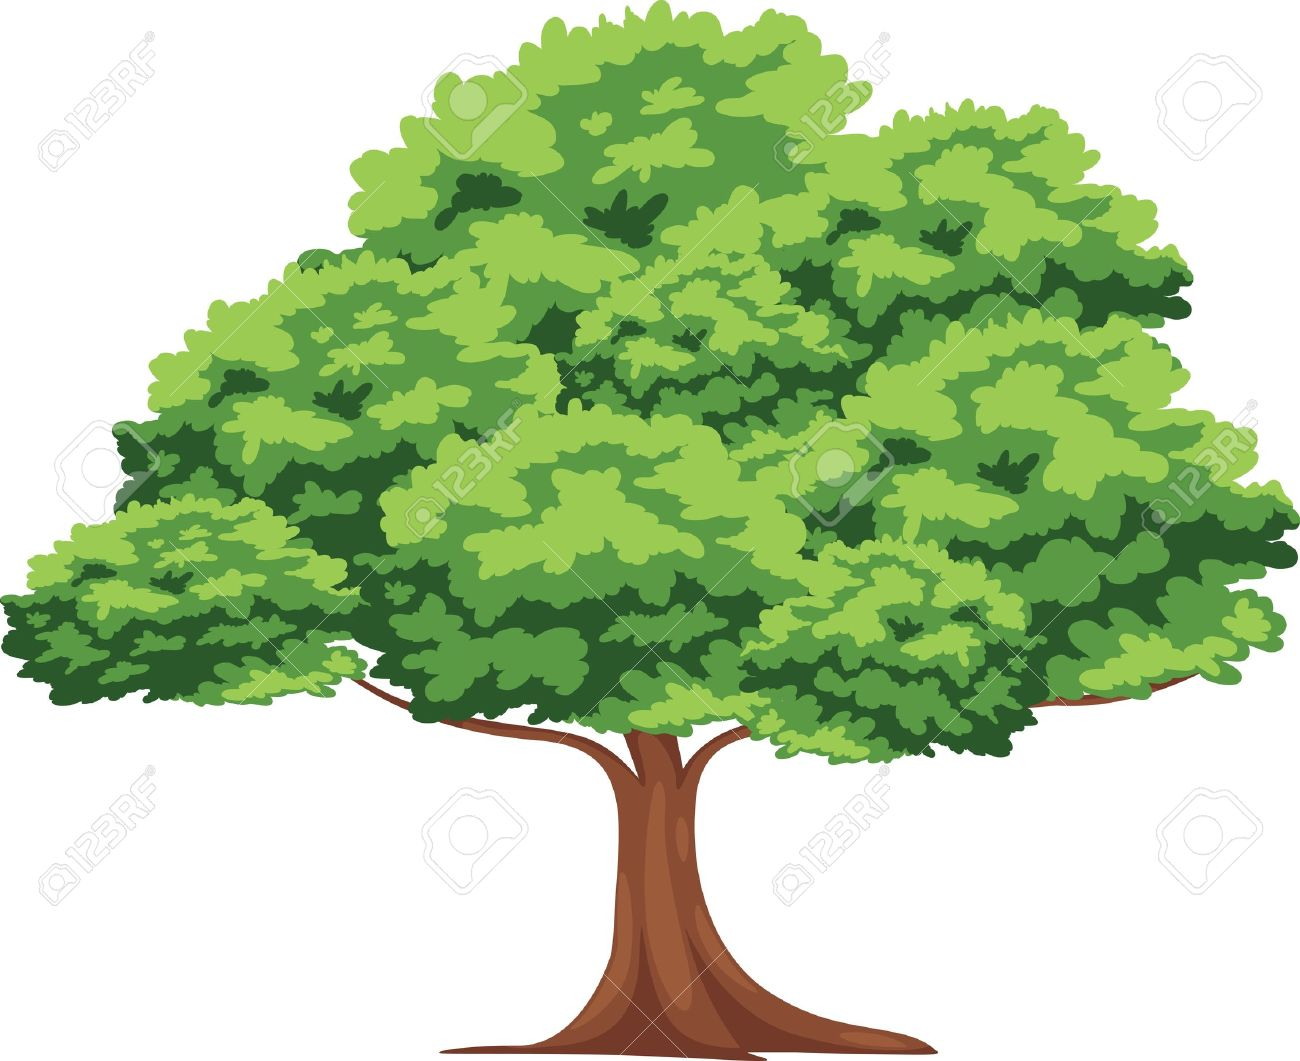
\includegraphics[width=\textwidth]{sample.jpg}
      \caption{} % Leave blank for just letter
      \label{fig2:doubleImage:b}
    \end{subfigure}
    \caption{This is an example of a double image figure.}
    \label{fig2:doubleImage}
  \end{figure}
  
  \begin{figure}[!htb]
    \centering
    \hspace*{\fill}% Adds space to left of top image (prevents two images from going to top)
    \begin{subfigure}{0.45\textwidth}
      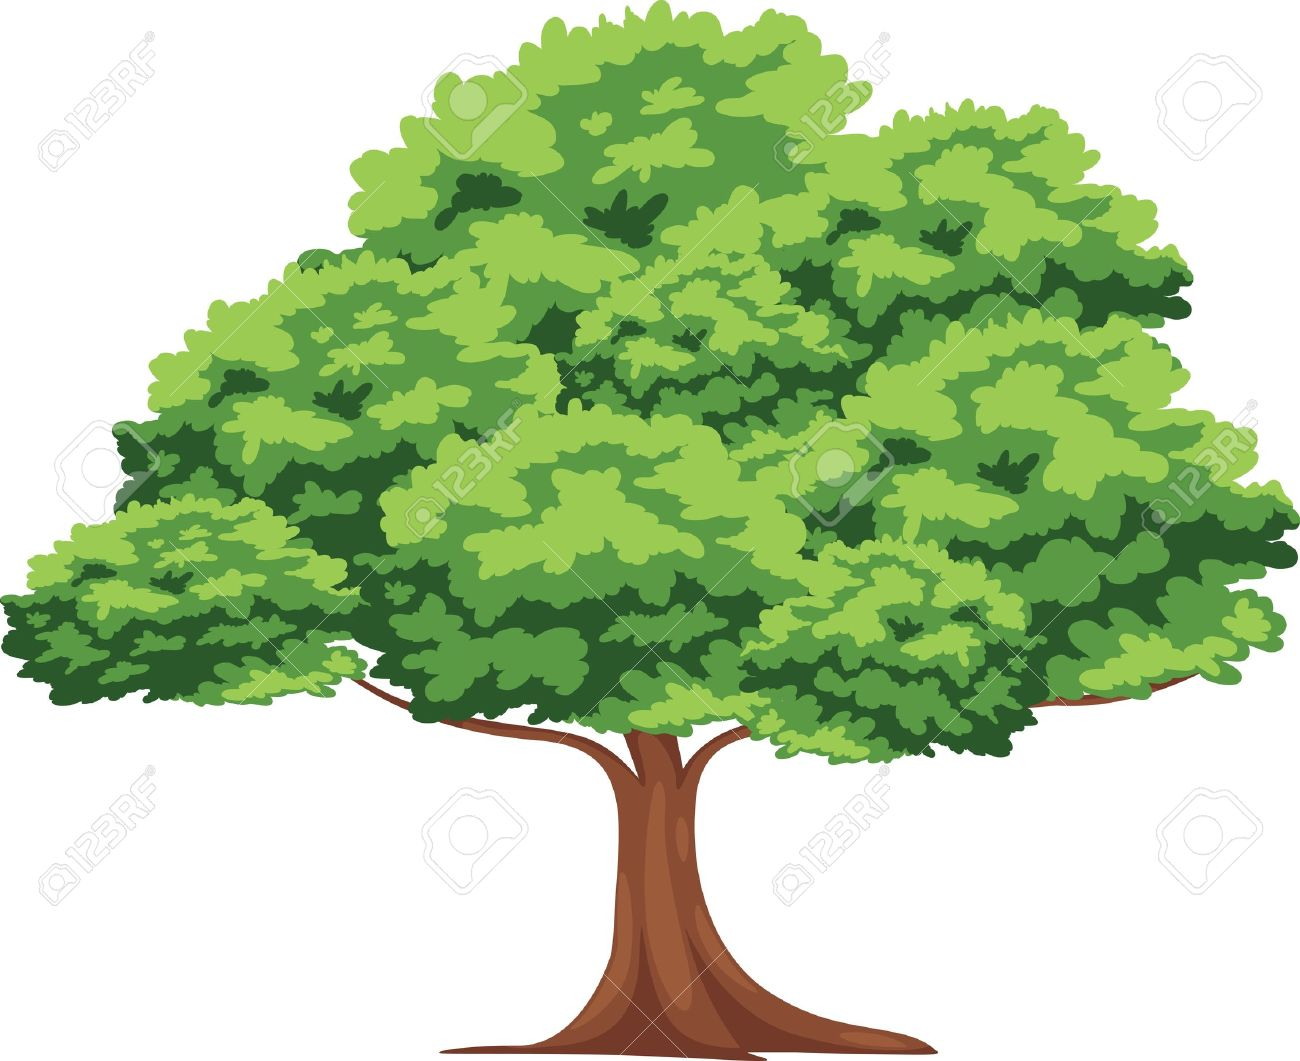
\includegraphics[width=\textwidth]{sample.jpg}
      \caption{} % Leave blank for just letter
      \label{fig3:tripleImage:a}
    \end{subfigure}
    \hspace*{\fill} % Adds space to right of top image (prevents two images from going to top)
    \par\vspace{1em}% Adds space between upper and lower images
    \begin{subfigure}{0.45\textwidth}
      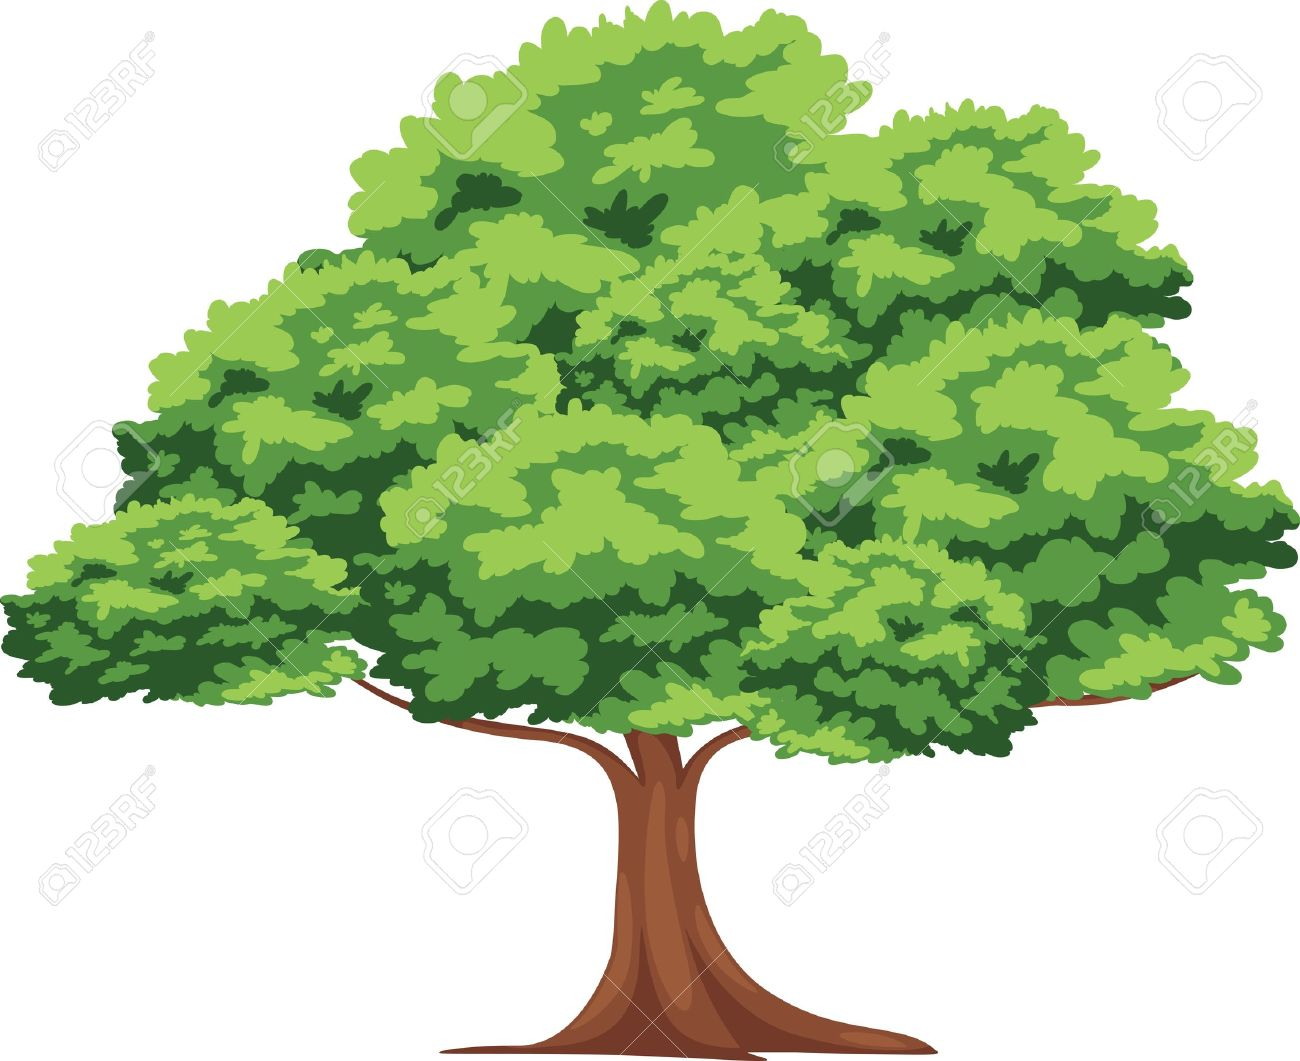
\includegraphics[width=\textwidth]{sample.jpg}
      \caption{} % Leave blank for just letter
      \label{fig3:tripleImage:b}
    \end{subfigure}
    ~ % Adds space between the two lower figures
    \begin{subfigure}{0.45\textwidth}
      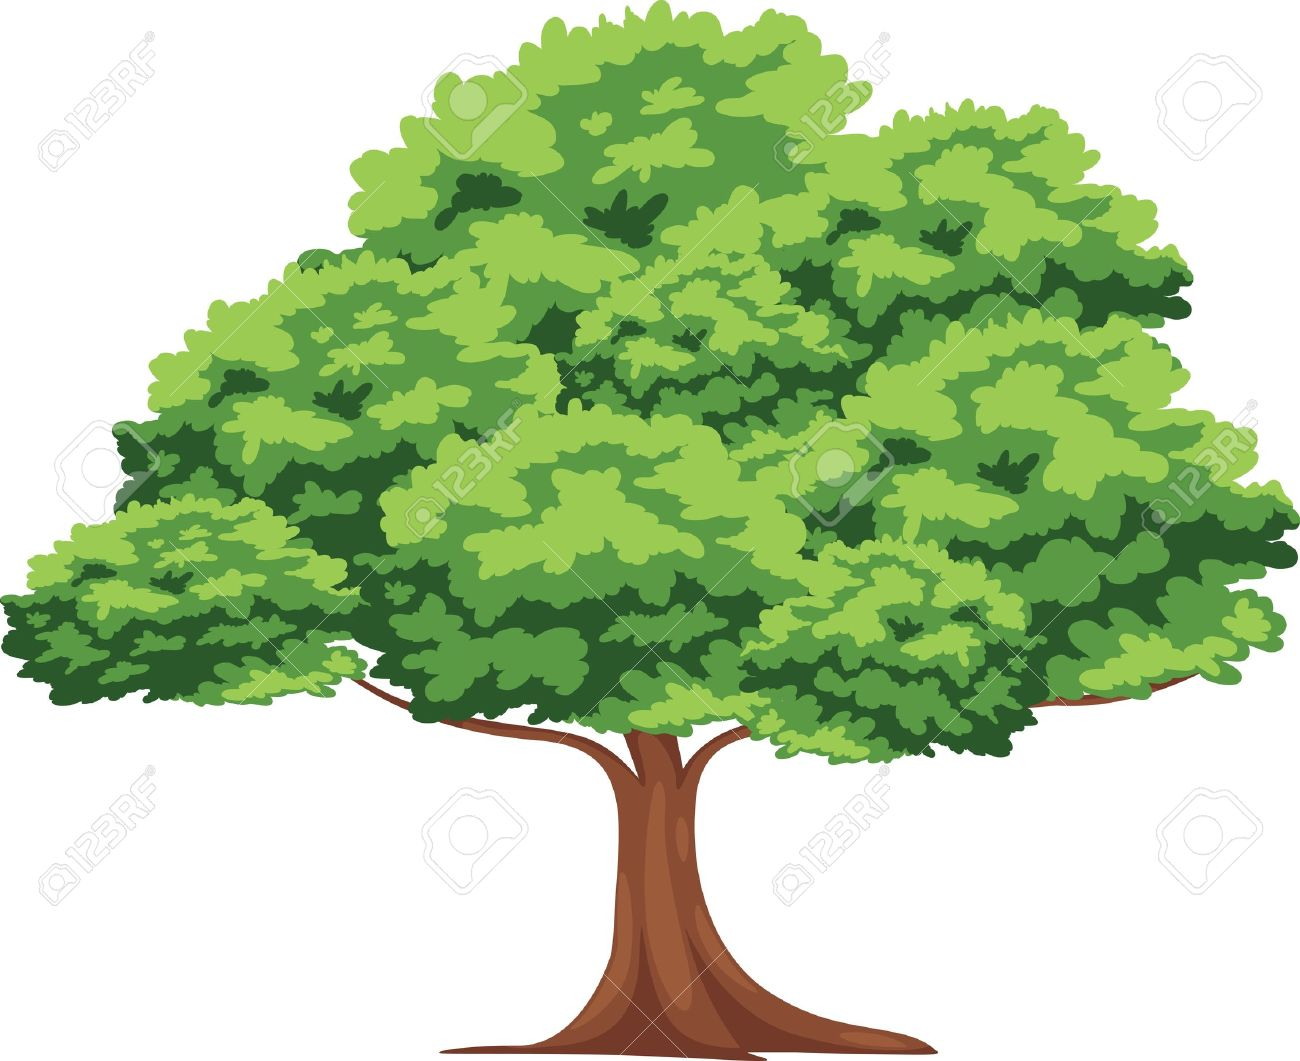
\includegraphics[width=\textwidth]{sample.jpg}
      \caption{} % Leave blank for just letter
      \label{fig3:tripleImage:c}
    \end{subfigure}
    \caption{This is an example of a triple image figure.}
    \label{fig3:tripleImage}
  \end{figure}
  
  \begin{figure}[!htb]
    \centering
    \hspace*{\fill}% Adds space to left of top image (prevents two images from going to top)
    \begin{subfigure}{0.90\textwidth+1em} % 0.9 = 0.45 + 0.45, and 1em is the width of ~
      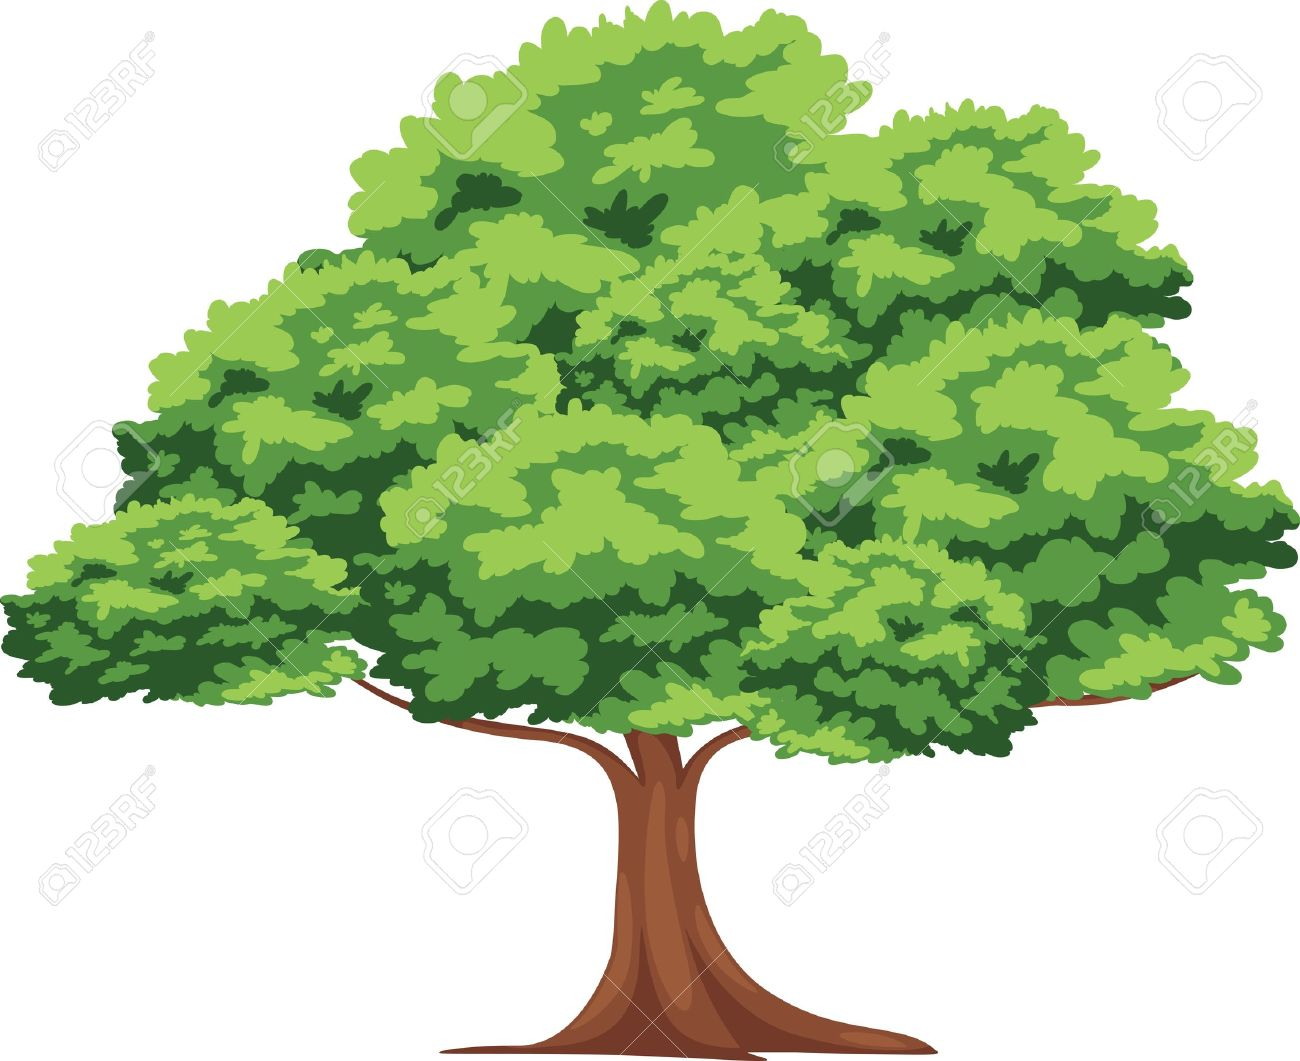
\includegraphics[width=\textwidth]{sample.jpg}
      \caption{} % Leave blank for just letter
      \label{fig4:tripleImage:a}
    \end{subfigure}
    \hspace*{\fill} % Adds space to right of top image (prevents two images from going to top)
    \par\vspace{1em}% Adds space between upper and lower images
    \begin{subfigure}{0.45\textwidth}
      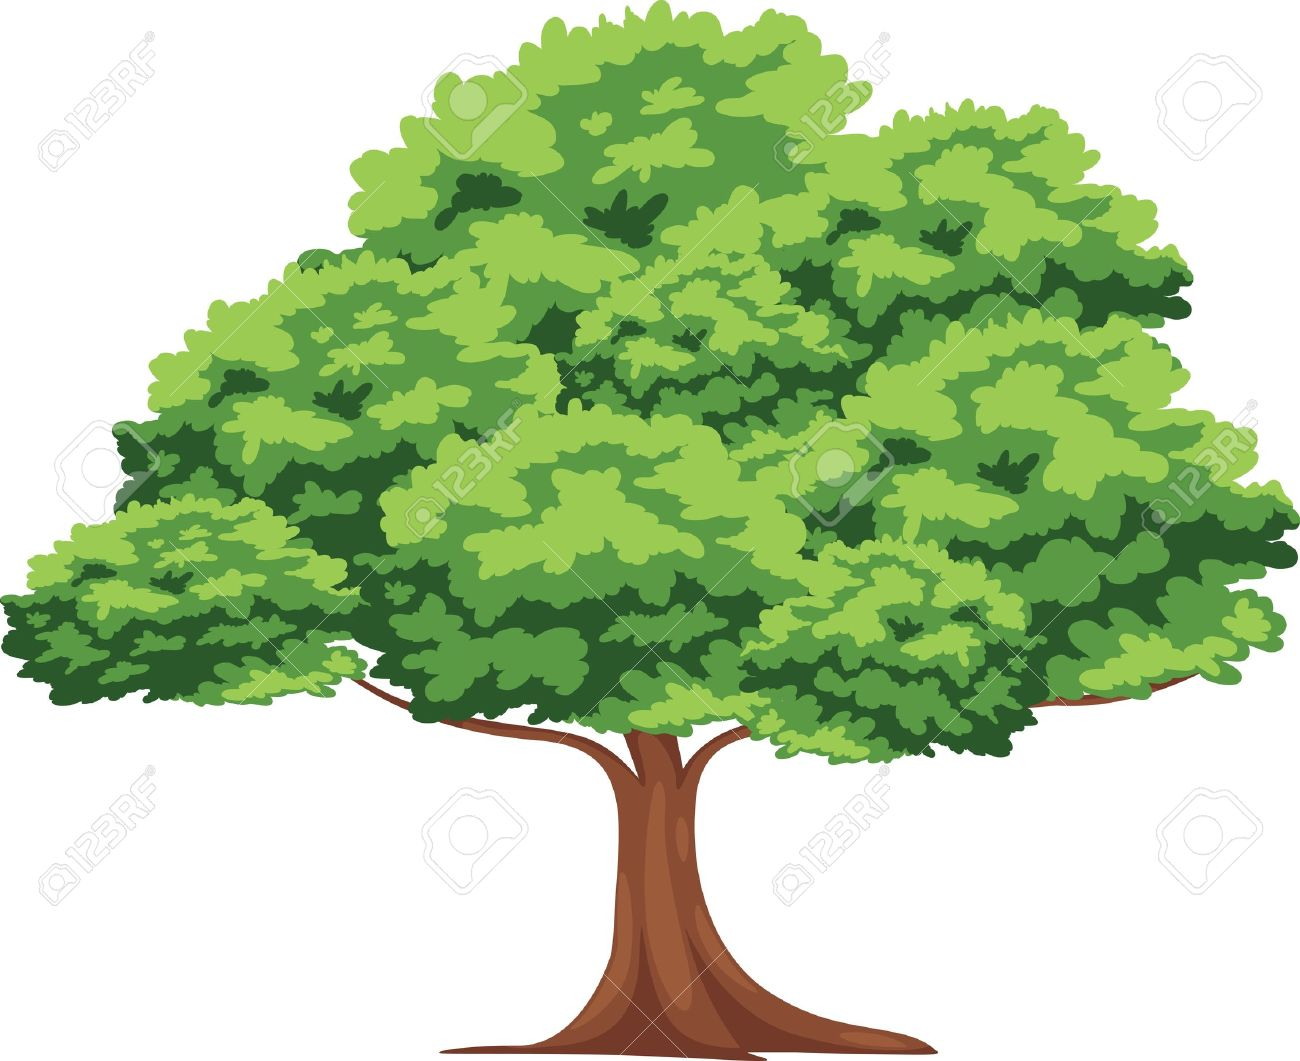
\includegraphics[width=\textwidth]{sample.jpg}
      \caption{} % Leave blank for just letter
      \label{fig4:tripleImage:b}
    \end{subfigure}
    ~ % Adds space between the two lower figures
    \begin{subfigure}{0.45\textwidth}
      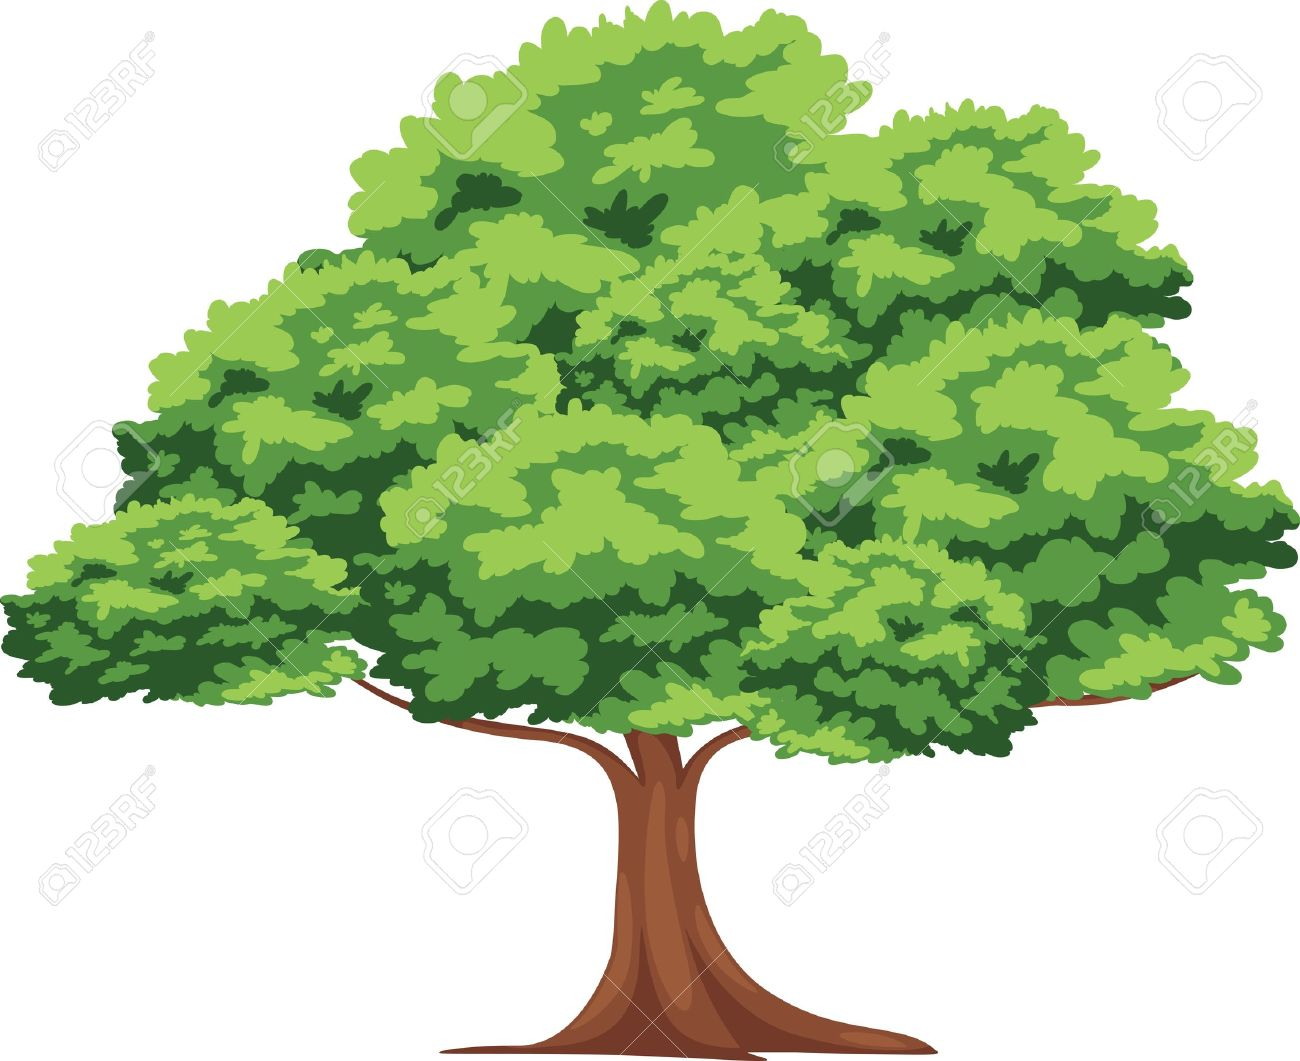
\includegraphics[width=\textwidth]{sample.jpg}
      \caption{} % Leave blank for just letter
      \label{fig4:tripleImage:c}
    \end{subfigure}
    \caption{This is a second example of a triple image figure.}
    \label{fig4:tripleImage}
  \end{figure}
  
  \begin{figure}[!htb]
    \centering
    \begin{subfigure}{0.45\textwidth}
      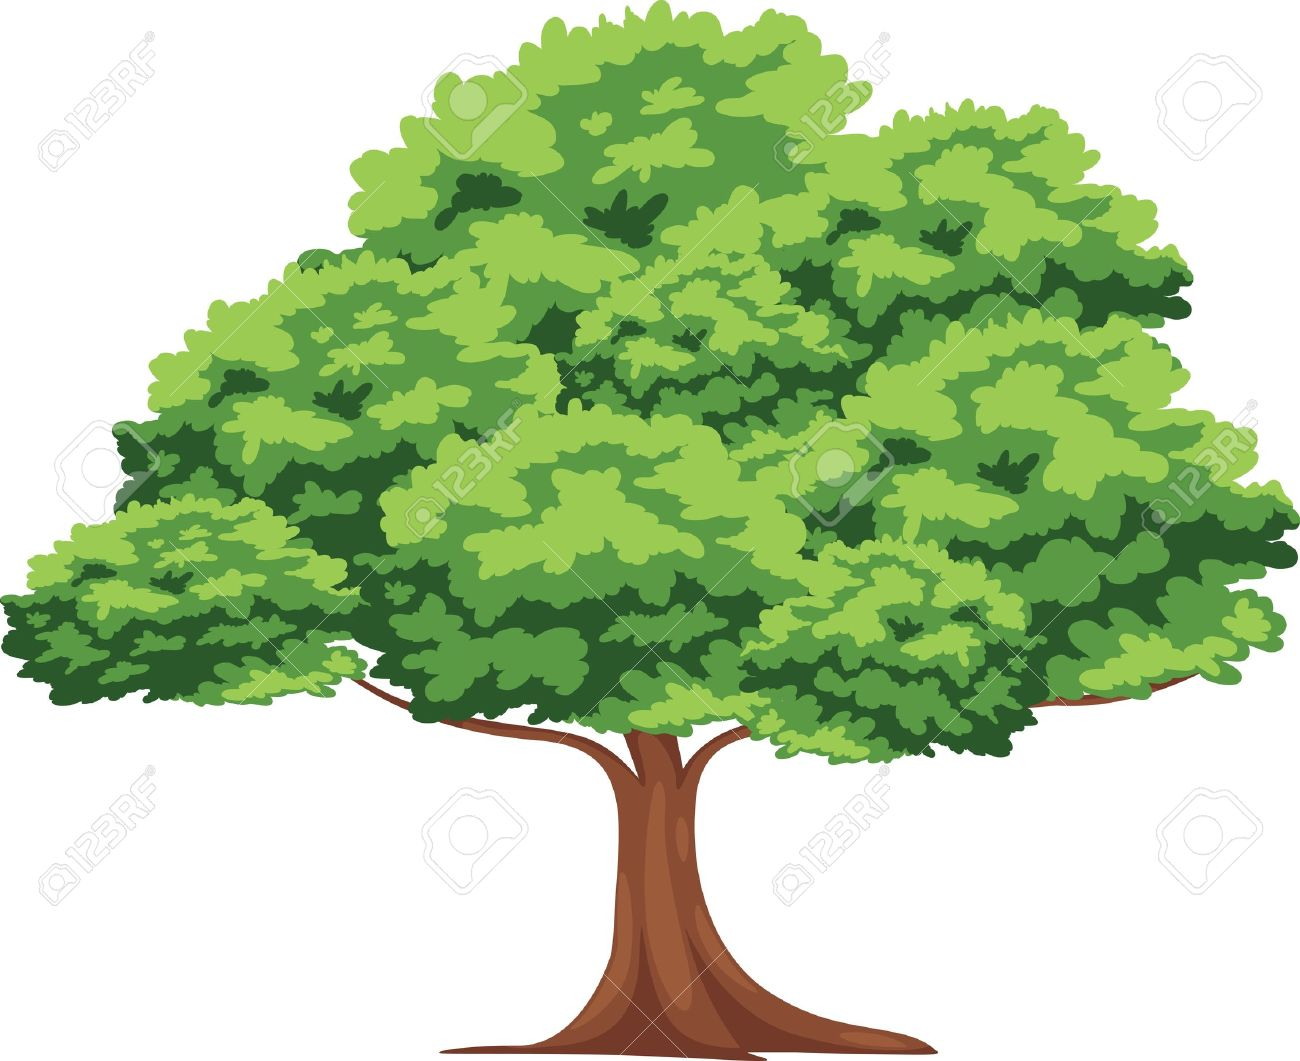
\includegraphics[width=\textwidth]{sample.jpg}
      \caption{} % Leave blank for just letter
      \label{fig5:quadImage:a}
    \end{subfigure}
    ~ % Adds space between the two top figures
    \begin{subfigure}{0.45\textwidth}
      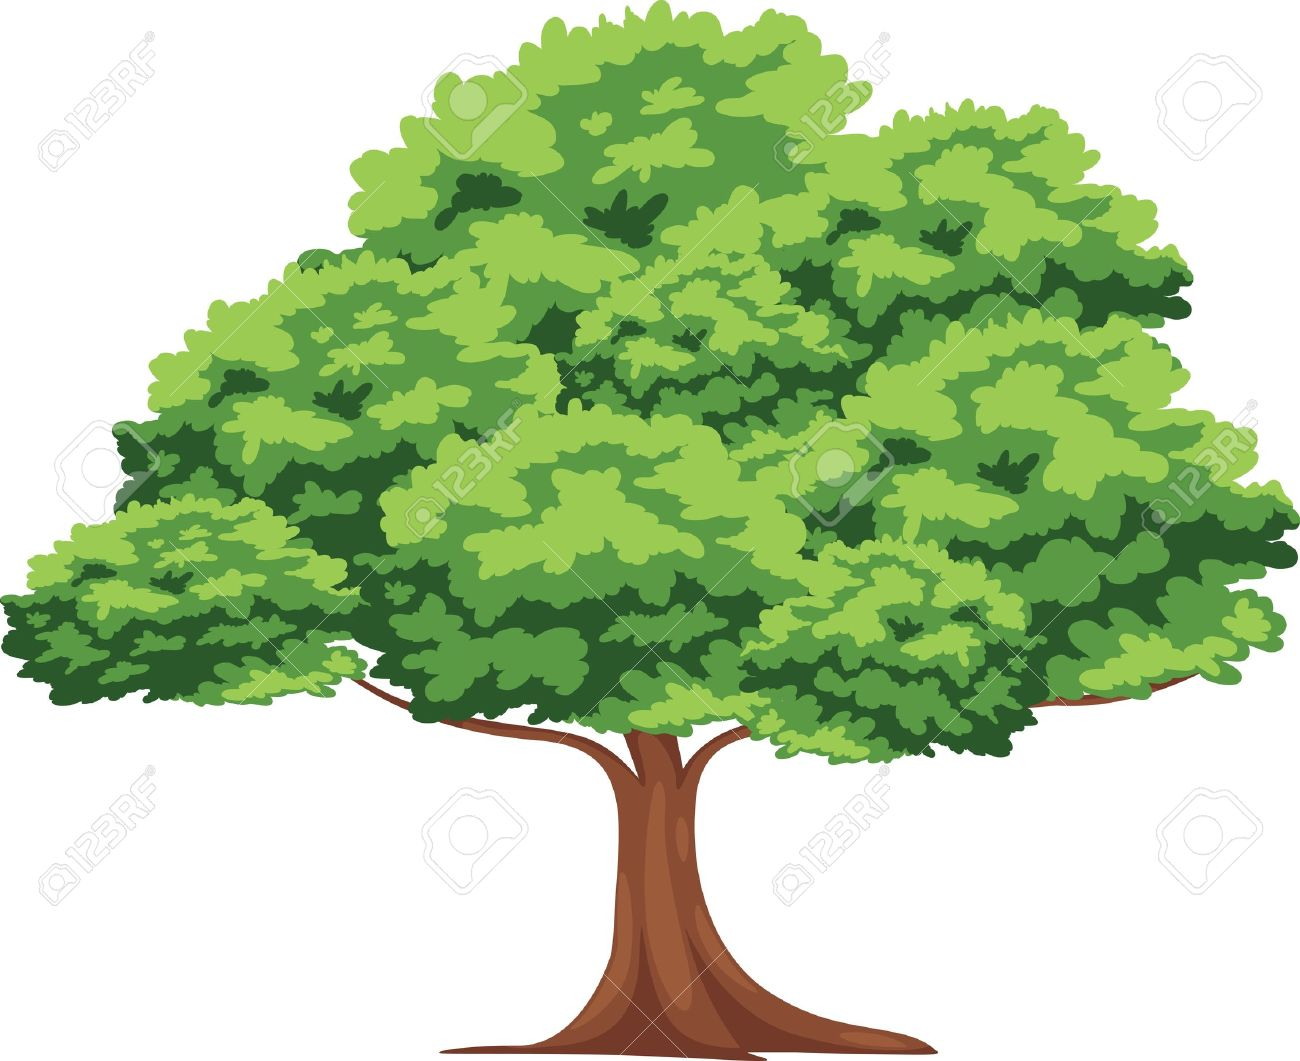
\includegraphics[width=\textwidth]{sample.jpg}
      \caption{} % Leave blank for just letter
      \label{fig5:quadImage:b}
    \end{subfigure}
    \par\vspace{1em} % Adds space between upper and lower images
    \begin{subfigure}{0.45\textwidth}
      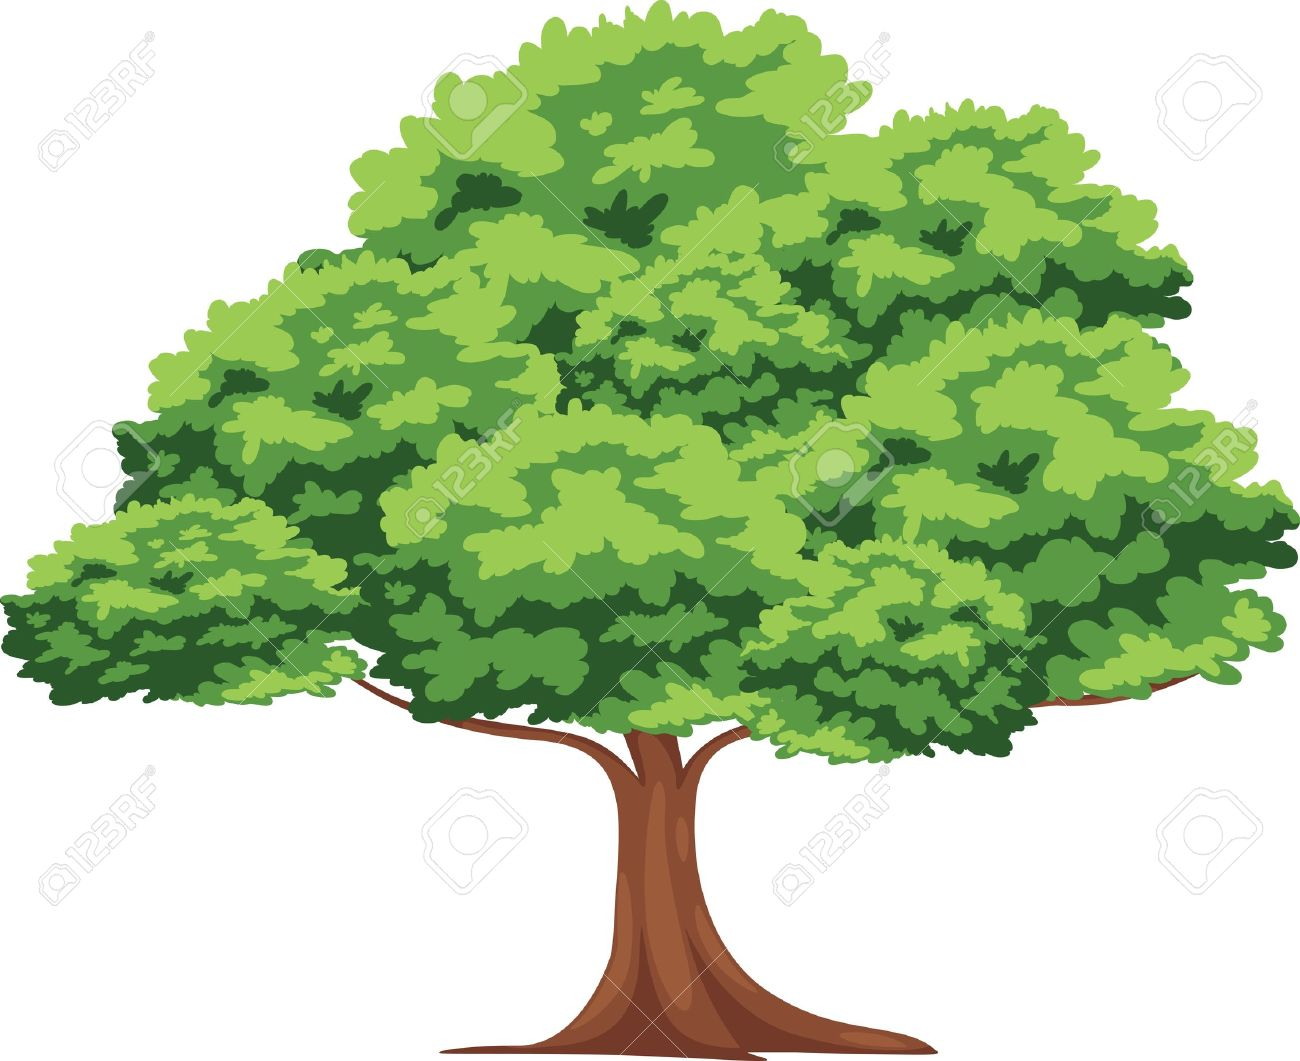
\includegraphics[width=\textwidth]{sample.jpg}
      \caption{} % Leave blank for just letter
      \label{fig5:quadImage:c}
    \end{subfigure}
    ~ % Adds space between the two lower figures
    \begin{subfigure}{0.45\textwidth}
      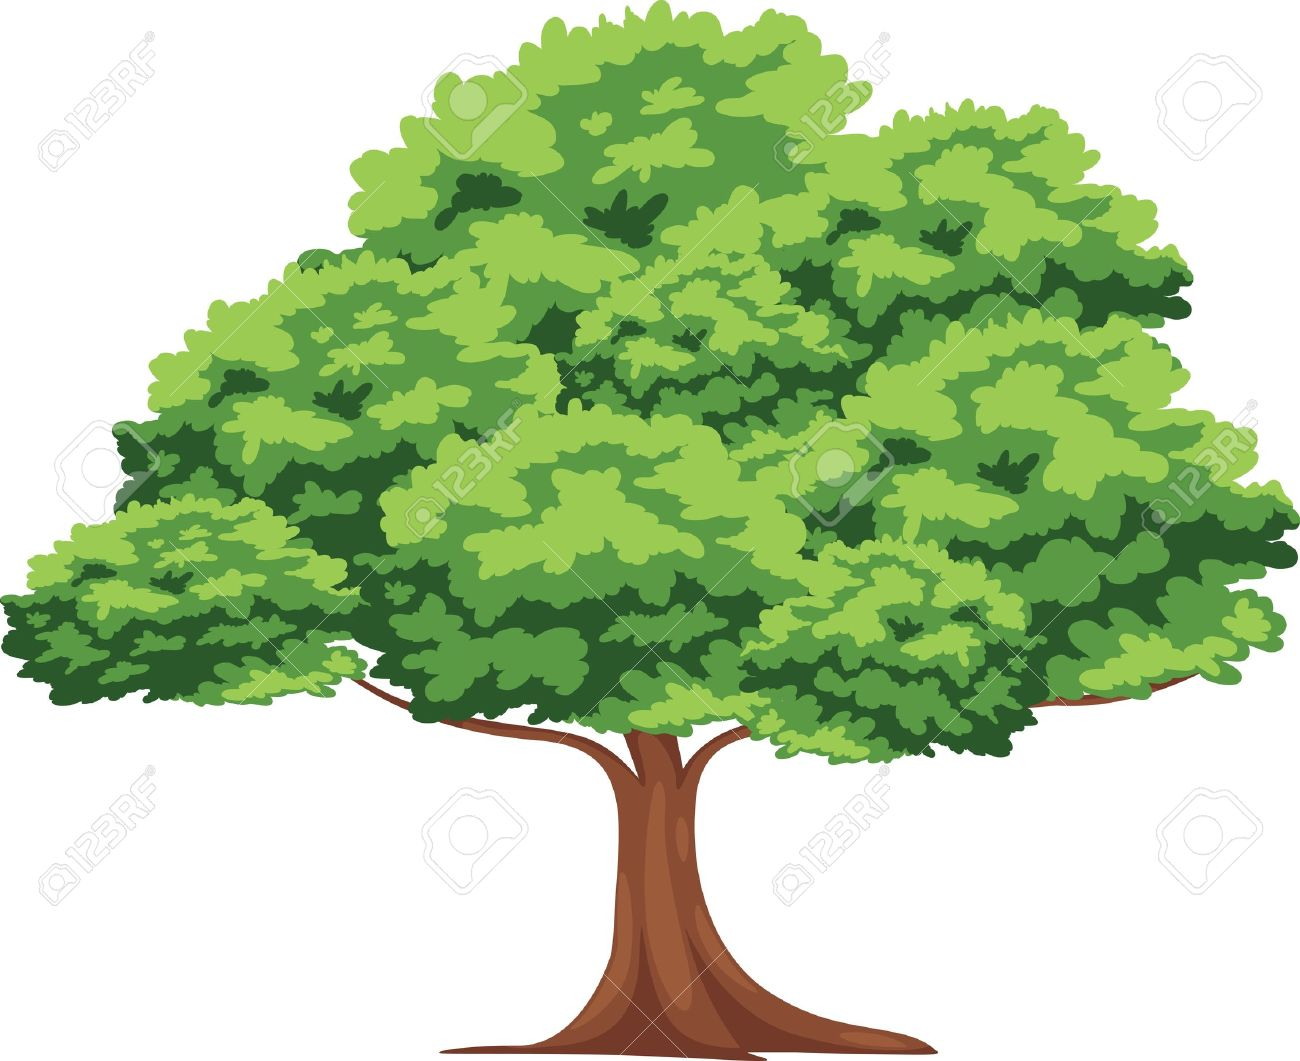
\includegraphics[width=\textwidth]{sample.jpg}
      \caption{} % Leave blank for just letter
      \label{fig5:quadImage:d}
    \end{subfigure}
    \caption{This is an example of a quad image figure.}
    \label{fig5:quadImage}
  \end{figure}
  
  \clearpage % forces the remaining images (floats to be placed)
  \section{Equations}
  The following equation has no referencing number:
  \nonumeq{E = & m\ c^2}
  
  \Cref{eq:quickEq} has a reference to it though. Or for more control the source for \Cref{eq:quickEq} can be written out fully as it was for \Cref{eq:quickEq2}.
  
  \numeq{pi = & 3.1415...}{eq:quickEq} % shorthand for the following way of writing equations.
  \begin{align}\label{eq:quickEq2}
    e = & 2.7183...
  \end{align}
  
  If you have multiple equations that you want arranged very neatly, use the align environment and you can assign individual equations numbers as shown in \Cref{eq:multiref:a,eq:multiref:b,eq:multiref:c}.
  \begin{align}%Note: Alignment happens at the "=" character
    \label{eq:multiref:a} Equation1 = & 1 + 1\\
    \label{eq:multiref:b} Equation2 = & 2 + 2\\
    \label{eq:multiref:c} Equation3 = & 3 + 3
  \end{align}
  
  
  
  \printreferences % Add a Reference Section to the end of the Chapter.

\section{Summary}

\chapter{Title of Chapter 3}\label{ch:ch3}

\lipsum
\chapter{Title of Chapter 4}\label{ch:ch4}

\lipsum
\chapter{Conclusion}\label{ch:Conclusions}

\section{Summary}
The main goal of this thesis was to ...

First, in Chapter \ref{ch:background},  

Finally, ...

\section{Contributions}
 The list of original  accomplishments described in this thesis can be summarized as the following:
 \begin{itemize}
     \item First accomplishment ... 
     
     \item Second accomplishment ...
     
     \item Third accomplishment ...
     
     \item Fourth accomplishment ... 
     
     \item Etc ...
 \end{itemize}
 
 In conclusion, 

\section{Future Considerations}
Your future considerations intro ...

\begin{itemize}

    \item First future work ...
  
    \item Second future work ...
    
    \item Third future work ...
    
    \item Fourth future work ...
    
    \item Fifth future work ... 
    
\end{itemize}

\chapter*{Thesis Publication List (as of April 2020)}
\addcontentsline{toc}{chapter}{Thesis Publication List (as of April 2020)}

This section lists the academic contributions made during the course of this doctoral thesis, including journal papers, conference papers, and patents.

\section*{Thesis-Related Publications}
This section lists the refereed journals, patents, and conference papers published during the course of this thesis work which are directly related to the thesis objectives.

\subsection*{Journals}
\begin{enumerate}
    \item S. Deif and M. Daneshmand, “Long Array of Microwave Sensors for Real-Time Coating Defect Detection,” \textit{IEEE Trans. Microw. Theory Tech.}, 2020, doi: 10.1109/tmtt.2020.2973385.
    
\end{enumerate}

\subsection*{Patents}
\begin{enumerate}
	\item M. Daneshmand, S. Deif, M. H. Zarifi, and N. Vahabisani; "Sensor system for pipeline integrity monitoring,", \textit{20190293547}:A1 26-Sep-2019. 
\end{enumerate}

\subsection*{Conferences}
\begin{enumerate}
   \item S. Deif, B. Leier, M. Snow and M. Daneshmand; "Microwave Sensor Array for Corrosion Prediction in Steel Tank Bottoms,"  in \textit{2018 12th International Pipeline Conference}, Calgary, Alberta, Canada, September 2018.
 
\end{enumerate}

\section*{Miscellaneous Publication List}
This section lists the refereed academic papers published during the PhD program but not directly related to the thesis topic.

\subsection*{Journals}
\begin{enumerate}
	\item M. Benlamri, S. Deif, et al., “Planar microwave resonator with electrodeposited ZnO thin film for ultraviolet detection,” \textit{Semicond. Sci. Technol.}, vol. 35, no. 2, p. 025003, Feb. 2020.
\end{enumerate}





% End of thesis Bibliography Printing.
\printreferences 

\bigskip 
\clearpage\singlespacing

%%%%%%%%%%%%%%%%%%%%%%%%%%%%%%%%%%%%%%%%%%%%%%%%%%%%%%%%%%%%%%%%%%%%%%%%%%%%%%%%
%                                 BIBLIOGRAPHY                                 %
%%%%%%%%%%%%%%%%%%%%%%%%%%%%%%%%%%%%%%%%%%%%%%%%%%%%%%%%%%%%%%%%%%%%%%%%%%%%%%%%
%\nocite{*}  % Uncomment if you have a bibliography with work read but not cited
% \printbibliography[heading=bibintoc]
\printbibliography[heading=bibintoc]
\bigskip
%%%%%%%%%%%%%%%%%%%%%%%%%%%%%%%%%%%%%%%%%%%%%%%%%%%%%%%%%%%%%%%%%%%%%%%%%%%%%%%%
%                                  APPENDICES                                  %
%%%%%%%%%%%%%%%%%%%%%%%%%%%%%%%%%%%%%%%%%%%%%%%%%%%%%%%%%%%%%%%%%%%%%%%%%%%%%%%%
\appendix
\chapter{Patch on curvature simulation maybe}\label{app:}
  \section{Section 1}\label{sec:}
    \lipsum[34-36]
  \section{Section 2}\label{sec:}
    \lipsum[38]

\chapter{Matlab code for ch 5}\label{app:1}
  \section{Section 1}\label{sec:1}
    \lipsum[34-36]
  \section{Section 2}\label{sec:2}
    \lipsum[38]

\chapter{Third Appendix}\label{app:2}
  \section{Section 1}\label{sec:3}
    \lstinputlisting[caption=This is a caption for the inserted code,style=MatlabStyle]{"./Code/matlabCode.m"}
  \section{Section 2}\label{sec:4}
    \lstinputlisting[caption=This is a caption for the inserted code,style=CStyle]{"./Code/cCode.cpp"}
    
    
\insertappendix{PDF_Appendix}



\end{document}
